%\documentclass[review]{elsarticle}
\documentclass[5p]{elsarticle}


\usepackage{lineno,hyperref}
\usepackage[separate-uncertainty=true,multi-part-units=single]{siunitx}
\usepackage{color}
\modulolinenumbers[5]
\usepackage{mhchem}
\usepackage{enumitem}
%\usepackage{trackchanges}

\journal{Geomorphology}


\newcommand{\COMON}{\begin{color}{blue}}
\newcommand{\COMOFF}{\end{color}}

\newcommand{\alon}{\begin{color}{red}}
\newcommand{\aloff}{\end{color}}

%% APA style
\bibliographystyle{model5-names}\biboptions{authoryear}

%\addeditor{Alain}

%%%%%%%
% The trackchanges package adds five new LaTeX commands:
%
%  \note[editor]{The note}
%  \annote[editor]{Text to annotate}{The note}
%  \add[editor]{Text to add}
%  \remove[editor]{Text to remove}
%  \change[editor]{Text to remove}{Text to add}
%
% complete documentation is here: http://trackchanges.sourceforge.net/
%%%%%%%



\begin{document}


	\begin{frontmatter}

\title{Three-dimensional geophysical imaging of the Royal Arches Meadow Rock avalanche in Yosemite Valley, California}

%% Group authors per affiliation:
\author[Marcus]{Marcus Pacheco\corref{cor1}}
\address[Marcus]{California State University, Fresno}
\cortext[cor1]{Corresponding author.}
\ead{mvpacheco90@mail.fresnostate.edu}

\author[Alain]{Alain Plattner}
\address[Alain]{University of Alabama}

\author[Greg]{Greg Stock}
\address[Greg]{Yosemite National Park}

\author[Chris]{[Christopher Pluhar}
\address[Chris]{California State University, Fresno}



										\begin{abstract}
										

Rock avalanches have occurred intermittently in Yosemite Valley, California, since the retreat of glaciers at the end of the last ice age \~15 ka. The Royal Arches Meadow rock avalanche is an approximately 0.5 million m3 deposit of rock debris located in eastern Yosemite Valley. Cosmogenic beryllium-10 exposure ages of boulders on the deposit indicated that the rock avalanche occurred at 14.0 +- 0.3 ka, shortly after deglaciation. The interface between the rock avalanche deposit and the underlying fluvial, deltaic, and lacustrine sediments therefore provides an elevation marker for the valley surface at that time.To image this interface, we collected eight Ground Penetrating Radar (GPR) and five Electrical Resistivity Tomography (ERT) profiles longitudinally and transversely crossing the rock avalanche. Both methods are sensitive to the contrast between the granitic avalanche deposit and the underlying sediments. We identified multiple reflectors in the GPR data that are continuous across the profiles, while ERT inversion results along the same profiles showed resistive material (1k-8k ohm m) overlying relatively conductive material (<1k ohm m). By constraining ERT inversions with picked GPR reflectors, we identified a single GPR reflector that separates resistive material on top from relatively conductive material underneath. This reflector is approximately horizontal at an average elevation of ~1207 m. We interpret this interface as the bottom of the rock avalanche and hence as the surface of Yosemite Valley at the end of the last glaciation. Thus, 10 m of aggradation have occurred on the terrace adjacent to the rock avalanche since emplacement. Our findings help elucidate the rock avalanche runout dynamics and the postglacial sedimentation history of Yosemite Valley.

									\end{abstract}

					\begin{keyword}
GPR \sep ERT \sep Yosemite
%\texttt{elsarticle.cls}\sep \LaTeX\sep Elsevier \sep template
%\MSC[2010] 00-01\sep  99-00
					\end{keyword}

	\end{frontmatter}

%\linenumbers






\section{Introduction}

Large rock slope failures, such as rock avalanches are among the most efficient process changing mountainous landscapes \COMON (REFERENCES HERE) \COMOFF. In Yosemite Valley, located in Yosemite National park, rock slope failures not only poses a serious hazard to the nearly four million visitors received yearly, but also to the park infrastructure. In this project however, we explore a positive aspect of rock avalanches in Yosemite Valley. In Yosemite Valley, those postglacial massive rock debris deposits  are well preserved \COMON (REFERENCE HERE) \COMOFF, and can provide us with an elevation marker of the valley floor during the time that they occurred.  Hence, providing us with insights of the local postglacial sedimentation history.  
\bigskip



\subsection{Physical Setting}

Yosemite Valley was initially carved by fluvial incision, and latter deepened by several glaciation cycles over the past several million years. The most recent glaciation, locally known as Tioga glaciation, peaked between 28 000 and 17 000 years BP and only partially filled  Yosemite Valley (\cite{huber1987geologic}). Subsequently, Yosemite Valley is thought to have deglaciated by about 15,000 to 17,000 years ago (\cite{huber1987geologic};  \cite{Wieczorek+1996}.

The valley fill is mainly composed of lacustrine, deltaic, and fluvial sediments \COMON Reference here\COMOFF, has a depth of up to 600m \cite{gutenberg1956seismic}, and the current valley surface is a broad and flat flood plain meandered by the Merced River \cite{Wieczorek+1996}. Flanked by up to 1km tall and steep granitic rock faces (Stock & Uhrhammer, 2010).
\bigskip
    
    
    
\subsection{Slope Failures In Yosemite Valley}

Because of  the nearly vertical and sometimes overhanging walls, mass wasting events such as rock falls, rock slides, and debris flows are common in Yosemite Valley. Most of those deposits are concentrated relatively close to the cliffs where they originated. However, at ten locations in Yosemite Valley , rock debris have traveled hundreds of meters onto the valley \COMON(REFERENCE HERE)\COMOFF. Those deposits were termed Rock Avalanches, because of their distinct geomorphological expression, run out of hundreds of meters, and volumes in the hundreds of thousands of m3 \COMON(Stock 2014, Evans 2006,  Hungr 2014, Wieczorek 1998, Stock 2010, Stock 2011)\COMOFF. 
\bigskip


   
\subsection{Royal Arches Meadow Rock Avalanche - RAMRA}

The Royal Arches Meadow Rock Avalanche (RAMRA) lies in the eastern Yosemite Valley, inside Yosemite National Park in California, USA (Fig.~\ref{Study_Area}A). The RAMRA has a long runnout (XX meters) onto the valley (Fig.~\ref{Study_Area}B), with a hummocky morphology (Fig.~\ref{Study_Area}C), and boulders ranging from tens of centimeters to several meters tall (Fig.~\ref{Study_Area2}).


								   \begin{figure*}[h]

	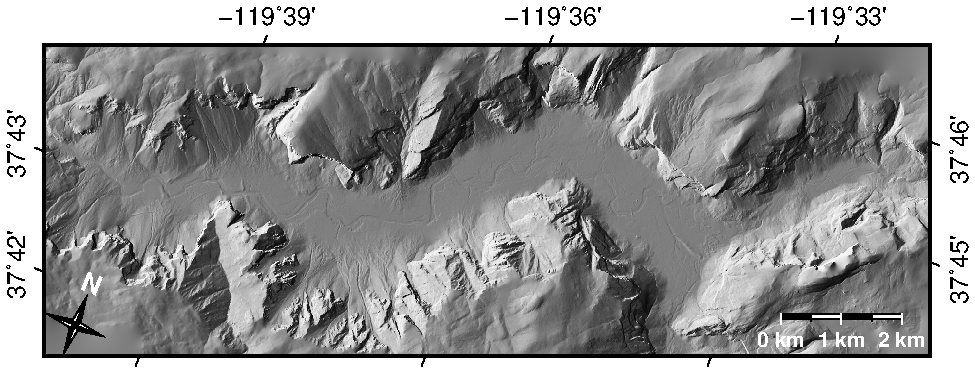
\includegraphics[width=\textwidth]{Yosemite.pdf}
		\caption{:(A) Yosemite Valley Map View, red box highlight the study area. (B) Zoom in the study area. (C) Topographic profiles across the study area.  \label{Study_Area}}

								   \end{figure*}




Generally, the size of the boulders decrease as you walk away from the cliff towards the Tenaya Creek (SW direction), until they completely disappear from the surface (Fig.~\ref{Study_Area}B). Because the valley has been aggrading in the last XX years \COMON reference here \COMOFF, it is possible that part of the Royal Arches Meadow rock avalanche has been covered. Here we refer to the exposed portion of the rock avalanche as the part of the rock avalanche that has visible signs of a large rock debris deposit containing boulders from tens of centimeters to several meters tall.   

                 
                                    \begin{figure*}[h]

	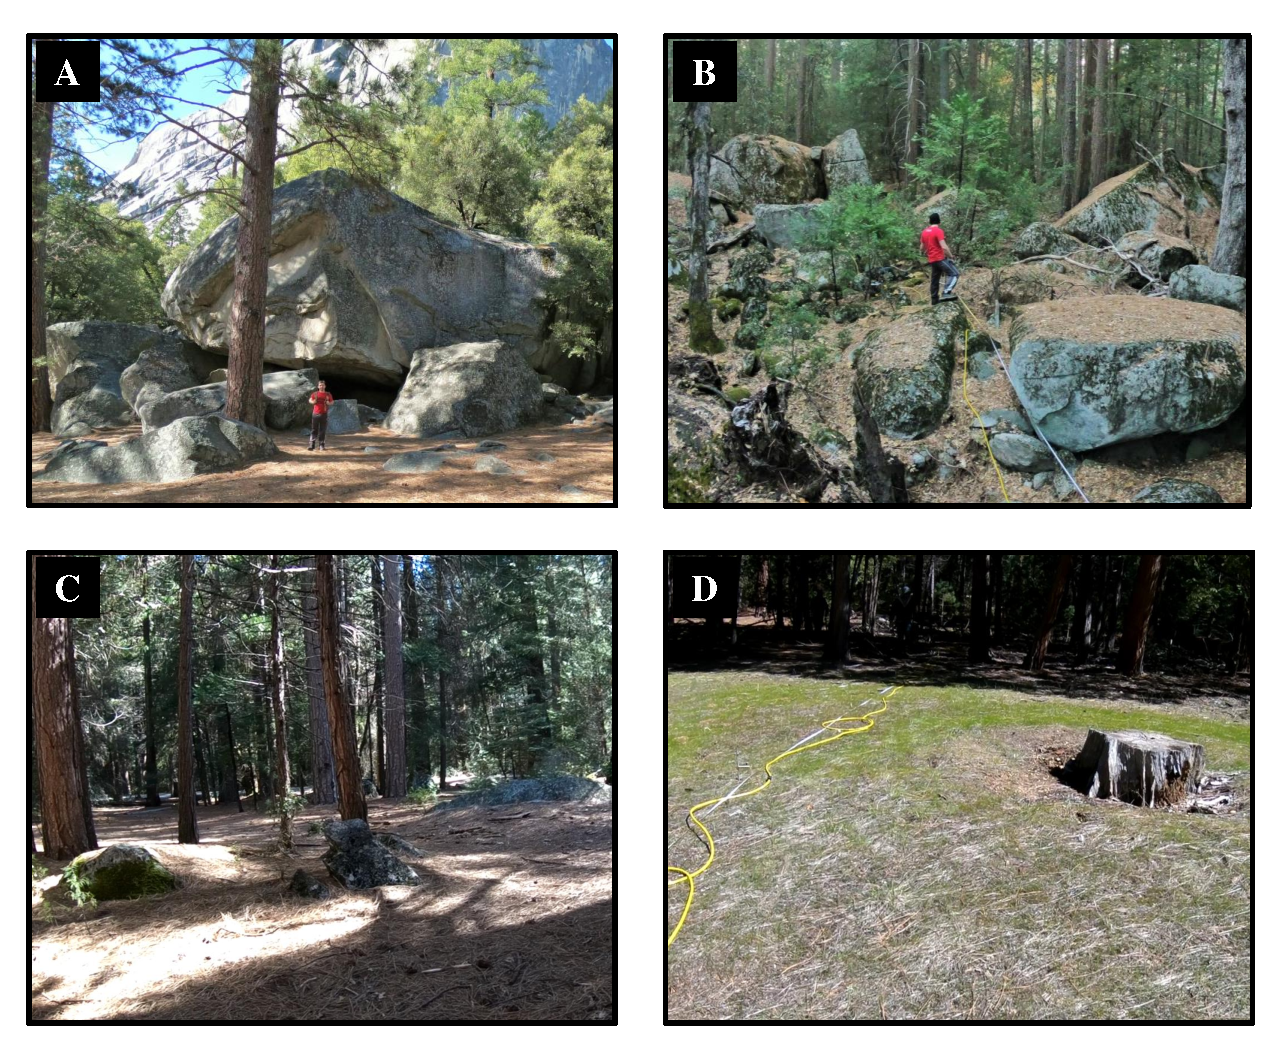
\includegraphics[width=\textwidth]{Study_Area2.pdf}
		\caption{: Large Boulders in the study area  \label{Study_Area2}}

								   \end{figure*}



Cosmogenic \COMON 10Be \COMOFF exposure ages demonstrate that the Royal Arches Meadow Rock Avalanche happened 14,030 ± 340 BP \COMON[XXX citation XXX]\COMOFF. This makes the RAMRA the oldest avalanche in the park. More importantly, because this event happened shortly after the LGM in the valley, the interface between the bottom of the RAMRA and the underlying paleo-valley marks the elevation state of the valley shortly after the LGM (15000 year B.P.). This boundary represent an important marker to understand the sedimentological evolution of the valley, and therefore, the target of study of this project.  

\bigskip

                 
                 
\subsection{Geophysics and Slope Failures Deposits}

To obtain spatially continuous information while minimizing impact, we used non-intrusive geophysical methods. Geophysical methods have been successfully applied to image slope failures deposits (e.g., \cite{sass2006determination}; \cite{otto2006comparing}; \cite{socco2010geophysical}; \cite{brody2015near},\cite{liu2018near}), highlighting the efficiency of combining different methods such as Electrical Resistivity Tomography (ERT) and Ground Penetrating Radar (GPR). 
                 
Ground Penetrating Radar is a geophysical technique that detects electrical discontinuities in the shallow subsurface (typically < 50 m) \citep{neal2004ground}. The most common form of GPR measurements, called common offset profiling, involves keeping a transmitter antenna and a receiver antenna at a fixed distance and moving them along a profile line on the surface to detect reflections from subsurface features \citep{jol2008ground}. Abrupt changes in dielectric permittivity caused by different lithologies, but also variations in grain size, and even grain orientation can reflect GPR waves (Olhoeft, G. R., 1998 and \citep{neal2004ground}. Therefore, we expect the contact between the bottom of the RAMRA with the underlying sediments to create strong reflections which can be detected by the GPR.          

Electrical Resistivity Tomography operates by measuring voltage differences caused by electric currents that are injected into the ground. Overlapping measurements can then, with the help of computational inversions, be turned into images of the electrical resistivity variation within the subsurface. These procedures are typically underdetermined. We hence can greatly improve the reliability of our solutions by providing additional constraints in the form for example of known interfaces (Oldenburg 1999; Loke 2013). We expect that this interface to be marked by a strong contrast in electrical resistivity, because the rock avalanche is composed of granitic debris (clast supported matrix), while the palleo-valley surface sediemntes are mostly composed of silt, clay, fine sands and soil. 

Doetsch, Linde, Pessognelli, Green, & Günther, (2012) \COMON cite this + add more references here! \COMOFF, have demonstrated the effectiveness of using Ground Penetrating Radar reflectors to constrain electrical resistivity tomography (ERT). This technique operates by offering the option of removing smoothness across the interfaces identified in the GPR data in the ERT inversion.  

\COMON Hi Alain, I am truing to create a connection between the last paragraph and the following one, I remember that you mentioned that it would be very important to state our goal here, therefore I would like to keep the "our goal is" to make it clear. \COMOFF

Our goal is to image the interface between the rock avalanche and the underlying valley surface using a a combination of Ground Penetrating Radar (GPR) and Electrical Resistivity Tomography (ERT).


\bigskip   





\section{Methods}

\subsection{Geophysics}


we collected Ground Penetrating Radar (GPR) and  Electrical Resistivity Tomography (ERT) profiles longitudinally and transversely crossing the rock avalanche.(Figure - Map). 

Because the extent of the rock avalanche is unknown, we positioned several profiles  inside the exposed portion of the rock avalanche. This way, we insured that we would be undoubtedly imaging the rock avalanche deposit just beneath the surface, and possibly its bottom. On the other hand, extending the geophysical profiles beyond the exposed portion of the rock avalanche,  allowed us to verify the lateral continuation of the bottom of the rock avalanche beyond its exposed portion. 

Eight GPR profiles were collected with a Sensors \& Software PulseEKKO Pro (\SI{50}{\mega Hz}) system (Fig.~\ref{GPR_ERT}a) during the months of September and October of 2018. Those profiles were then processed using GPRPy \citep{plattner2019comunity}. Processing flow and corrections included: time zero correction, filter (DEWOW and mean trace removal), T-pow gain, velocity analysis (based on WARR data), migration \citep{stolt1978migration} and topographic correction. We then used the processed profiles to track the lateral continuity of specific reflectors following the methodology proposed by \citep{mitchum1977seismic}.
	
Our vertical resolution (capacity to distinguish individual layers) is ___XX m. We estimated it using a velocity of 0.11m/ns (extracted from WARR data), a 50MHz frequency (used antenna), and the rule of thumb that vertical resolution is typical equals to a quarter of the wavelength. This estimation is useful to give us an idea of vertical resolution, but it still an approximation, since the physical properties of the medium (e.g. dielectric permitivity, electrical conductivity, and magnetic permitivity) can influence the vertical resolution \COMON (Cite____Olhoeft, G. R., 1998, Olhoeft, G. R., 1999; \citep{neal2004ground}) \COMOFF.


Five ERT transects were collected at the study area (Figure XX) using the Advanced Geosciences Inc SuperSting R1 (28 electrodes), with an electrode spacing of six meters, and a Wenner–Schlumberger and dipole-dipole acquisition scheme. Subsequently, the ERT data were filtered using DC2DInvRes \COMON (REFERENCE) \COMOFF and inverted using BERT/GIMLi (\cite{gunther2006three} and (\cite{Ruecker2017}).


\subsection{Cosmogenic beryllium-10 exposure ages}

-Cosmogenic be 10 in 3 locations
-Cosmogenic beryllium-10 ages yield a mean exposure age of 15.3 +- 1.4 ka


 
\section{Results}




\subsection{GPR Results}

By analyzing the processed GPR profiles, we identified three nearly horizontal continuous reflectors that are consistent along and across profiles (Fig.~\ref{GPR_Oblique}). -We named them Alpha, Beta, and Gamma.  And their average elevation can be found in table 1. 
. 

								 \begin{figure*}[h]

	\includegraphics[width=\textwidth]{Figures/GPR_Oblique.pdf}
		\caption{:(A) Oblique view of GPR profiles looking towards NW, (B) Tracked Reflectors Alpha, Beta, and Gamma, and (C) Interpolated surface for reflector Beta. \label{GPR_Oblique}}

								   \end{figure*}
								   
\begin{itemize}
    \item Table 1 here
\end{itemize}			   



We observed a pattern of three reflectors in different elevation, that presented a strong lateral continuity along and across profiles. Those sections of the GPR profiles can be described as following: (A )from the surface until approximately 1212m of elevation, the GPR profiles are marked by a plan-parallel reflectors to sub-parallel reflectors. Varying from 12YY until 12XX m of elevation, a strong plan-parallel reflector (Alpha) is visible in all GPR profiles.(B) Bellow ~1212 m of elevation the pattern of reflectors change to a chaotic geometry as the signal gets scattered. (C)In profiles A, B C, and D it is possible to identify a strong reflector at elevation of ~1207 m (Beta). and in a Gx,  Gy, Gz, GPR profiles another strong continuous reflector is identified at the elevation of ~1205m (Gamma).
								   
								   
								   
\subsection{ERT Results}

– we observed  in the ERT inversion results relative resistive material (1k-8k ohm m) overlying relatively conductive material (<1k ohm m).

\COMON Pictures? \COMOFF

And The ERT inversions using GPR reflectors for profiles E1, E2, E3, E4 and E5 have demonstrated that Reflector Beta best constrained the inversion, by creating a sharp interface between resistive/conductive material.


\COMON Pictures? \COMOFF


\COMON ________Combining the Methods____ \COMOFF


--Because of the difficulties imposed by the field of study (e.g. big boulders,  large fallen trunks) we were not able to collect a dense grid of geophysical data on the top of the rock avalanche. 

--We tried to collect as much geophysical data on the top of the rock avalanche as possible. However, difficulties imposed by the filed area, such as the dense presence of large boulders and/or big fallen trunks made the logistics for either GPR and/or ERT not practical. 

-To overcome the lack of one of the methods in specific locations we used the overall pattern of observation to predict how the data would look like in this area. 

- For example, we were not able to cover E5 entirely with GPR profiles, but we have a good idea where the elevation of the main reflectors would appear in this portion based on the elevation where they appear in the adjacent profiles.

-Similarly, in profile G5.1, we observed a strong signal attenuation below the elevation of 1212 m (Figure XX A). But we feel confident to picked the reflector named Beta here at the elevation of ~1207 meters based on: 
1) the weak rflction that appear among the attenuated signal at this elevation (Figure XX B).

2) the consistence in which Beta appears in the adjacent profiles at the elevation of approximately 1207m.

3) how well this picked reflector constrains the resistive/conductive transition at elevation of 1207m (Fig. XX C and D), annalagous to the other ERT constrained inverstions. 
								   
				(Fig.~\ref{Combined_ABCD})			

                                \begin{figure*}[h]

	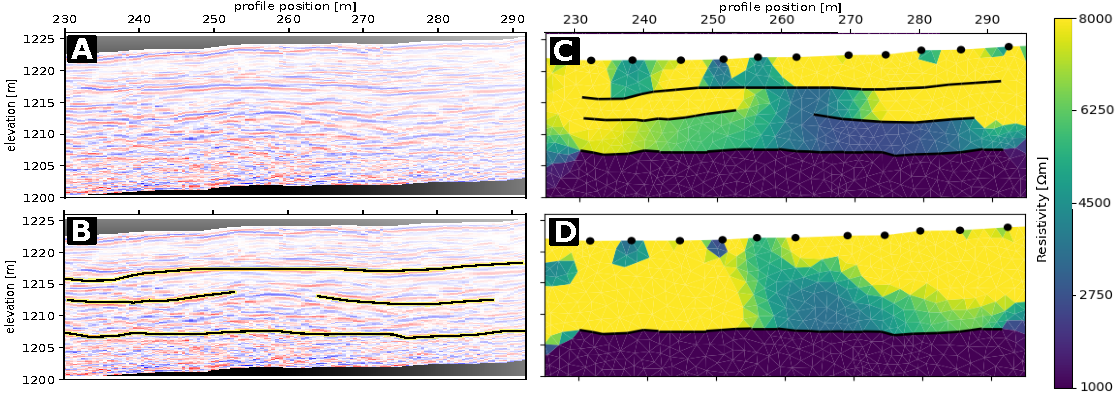
\includegraphics[width=\textwidth]{Figures/Combined_ABCD.pdf}
		\caption{:(A) Oblique view of GPR profiles looking towards NW, (B) Tracked Reflectors Alpha, Beta, and Gamma, and (C) Interpolated surface for reflector Beta. \label{Combined_ABCD}}

								   \end{figure*}





\section{Discussion}

- We interpreted Beta as the bottom of the rock avalanche. Because: 

	(1) This is the Reflector that best constrain the ERT Inversion (transition between resistive / 	conductive) is the interface between the bottom of the rock avalanche


- Discuss reflector configuration (dipping, energy scatter, etc) 


- Proxy for the palleo-valley (paleoelevation)  surface of yosemite valey shortly after the last glacial maximum (LGM).



\subsection{Aggradation Rate since the LGM}

We interpret this interface as the bottom of the rock avalanche and hence as the surface of Yosemite Valley at the end of the last glaciation; thus,   10 m of fluvial sedimentation has occurred at this site over the past 14 ka




\subsection{Volume}

-Distal volume estimation considering the bottom of the rock avalanche as the present valley floor =  378,000 m3

-Distal volume estimation considering the bottom of the rock avalanche as the interpreted bottom of the rock avalanche from the geophysical data = 955,000 m3 

-This is not the total volume of the avalanche, but it demostrate how estimations based on purely surface intereprations can be off. Mainly in environments dominated by aggradation. 





\section{Conclusions}

-The combination of GPR and ERT has proven to be a powerful tool to image the interface between the RAMRA and the underneath valley sediments. 


-GPR resolution along with GPR and ERT depth sounding was satisfactory considering the goal of this project. 

-Geophysical data was consistent.
	-Different and isolated data processing show similar results when comparing different profiles and different methods. 


-rock avalanche risk assessment improvement 
	volume estimation based on purely surficial data might lead reasearchhers to underestimation


\section{acknowledgements}






\bibliography{mybibfile}

\end{document}